% !TeX TS-program = xelatex

\documentclass{beamer}

\usepackage{tabularx}
\usepackage{xltxtra}
\usepackage{fontspec}
\usepackage{polyglossia}
\usepackage{makecell}
\usepackage{listings}
\usepackage{pifont}
\usepackage{xcolor}

\usepackage{circuitikz}
\usepackage{tikz}
\usetikzlibrary{arrows.meta,calc,decorations.markings,math,arrows.meta,shapes,arrows,decorations.pathreplacing}
\usetikzlibrary{positioning}

\tikzset{block/.style = {draw, fill=white, rectangle,
		minimum height=3em, minimum width=2cm},
	input/.style = {coordinate},
	output/.style = {coordinate},
	pinstyle/.style = {pin edge={to-,t,black}},
	radiation/.style={decorate,decoration={expanding waves,angle=12,segment length=4pt}}
}

\setbeamertemplate{endpage}{%
	\begin{frame}
		\begin{center}
			\Huge Demo
		\end{center}
	\end{frame}
}

\definecolor{mGreen}{rgb}{0,0.6,0}
\definecolor{mGray}{rgb}{0.5,0.5,0.5}
\definecolor{mPurple}{rgb}{0.58,0,0.82}
\definecolor{backgroundColour}{rgb}{0.95,0.95,0.92}

\lstdefinestyle{CStyle}{
    backgroundcolor=\color{backgroundColour},   
    commentstyle=\color{mGreen},
    keywordstyle=\color{magenta},
    numberstyle=\tiny\color{mGray},
    stringstyle=\color{mPurple},
    basicstyle=\footnotesize,
    breakatwhitespace=false,         
    breaklines=true,                 
    captionpos=b,                    
    keepspaces=true,                 
    numbers=left,                    
    numbersep=2pt,                  
    showspaces=false,                
    showstringspaces=false,
    showtabs=false,                  
    tabsize=2,
    language=C
}


\setdefaultlanguage{german}

\usetheme[blue]{Verona}
\usefonttheme{default}
\usefonttheme{professionalfonts}

\usefonttheme[stillsansseriftext]{serif}

\defaultfontfeatures{Ligatures=TeX,Scale=MatchLowercase}


\title{Asynchronous DRAM over SPI}
\subtitle{Implementierung eines DRAM-Controllers mit Web-API}
\author{Maximilian Gaul}
\date{04.02.2020}

%\mode<presentation>

\begin{document}
	
\begin{frame}
	\titlepage
\end{frame}

\begin{frame}

	\frametitle{Das PCB}
	\framesubtitle{Schematic}
	\begin{center}
		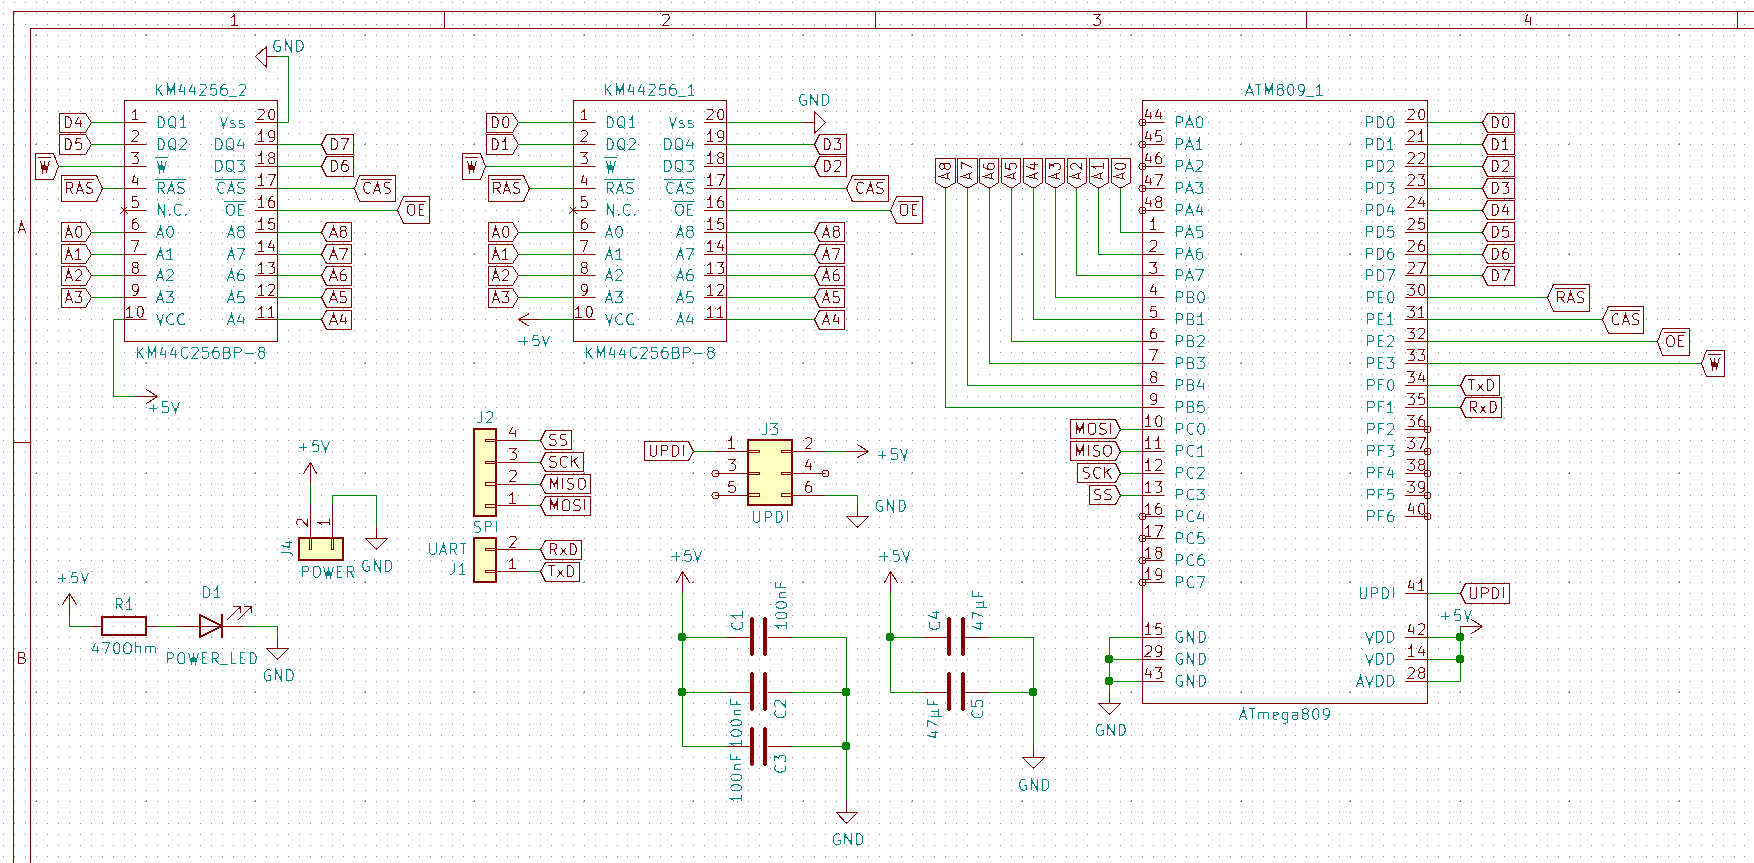
\includegraphics[scale=0.243]{images/KiCAD_Schematic_View.png}
	\end{center}

\end{frame}

\begin{frame}

	\frametitle{Das PCB}
	\framesubtitle{Layout}
	\begin{center}
		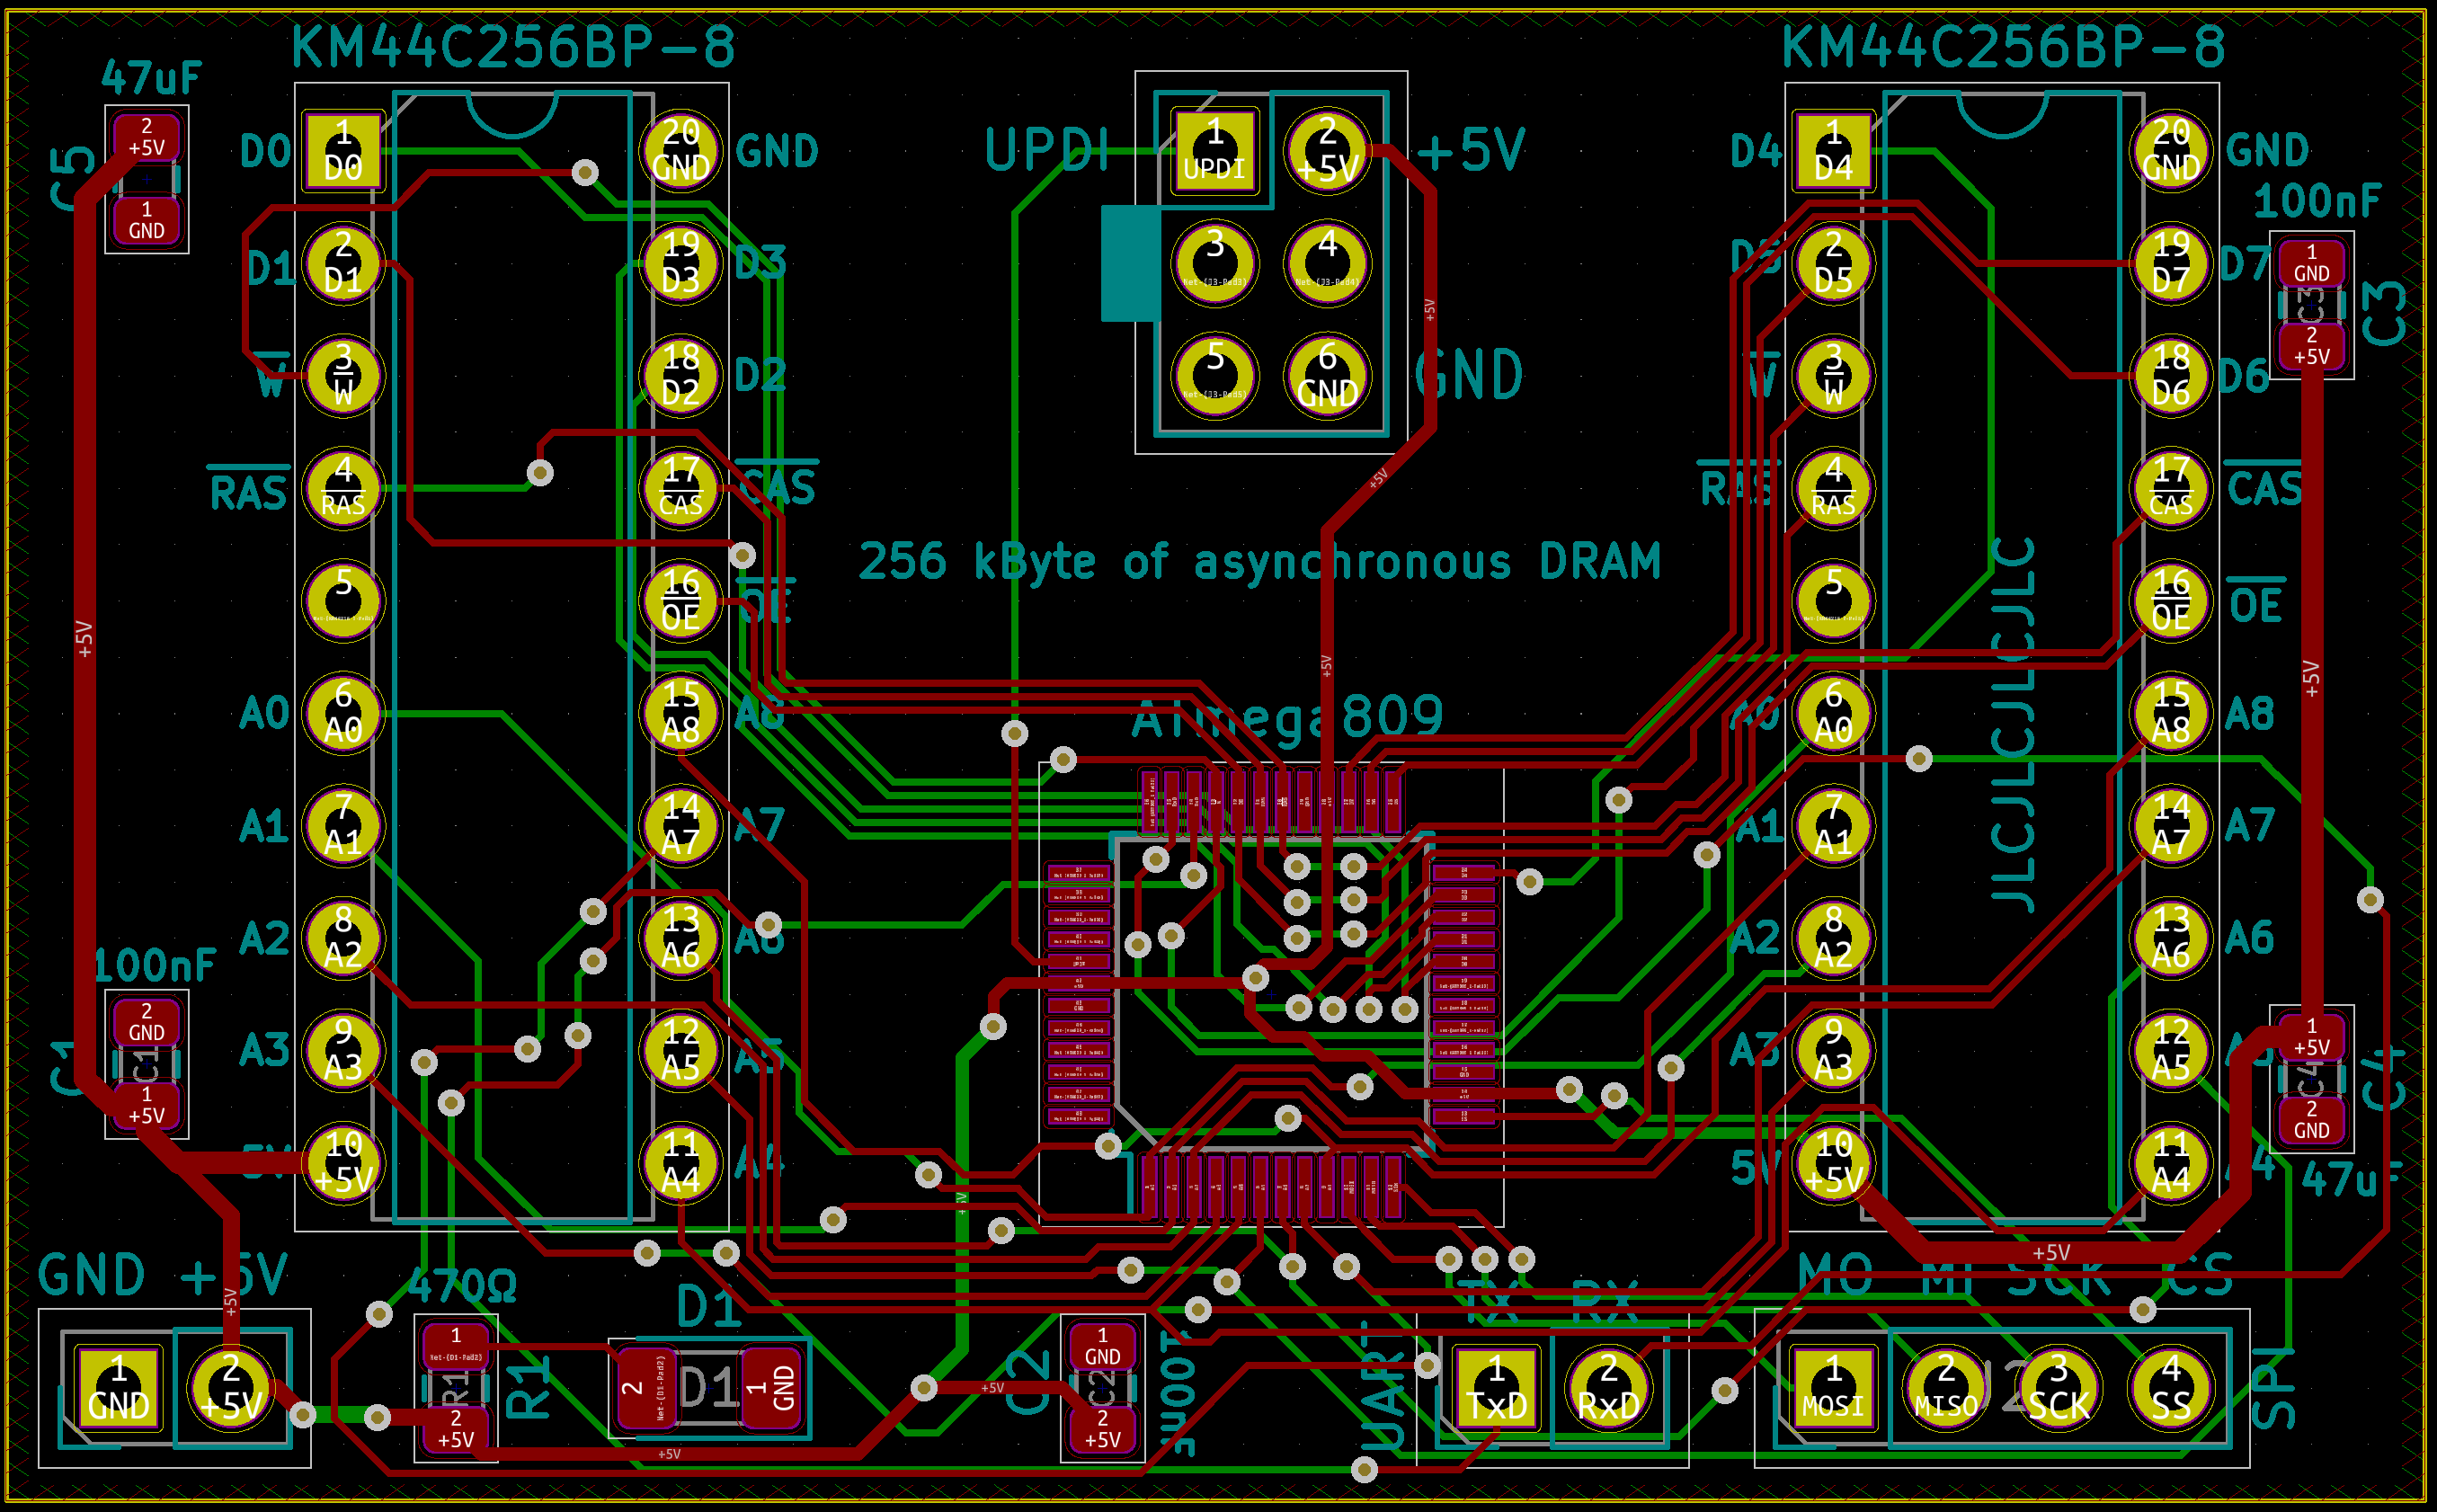
\includegraphics[scale=0.15]{images/KiCAD_2D_PCB_View.png}
	\end{center}
	
\end{frame}

\begin{frame}

	\frametitle{Das PCB}
	\framesubtitle{Layout}
	\begin{center}
		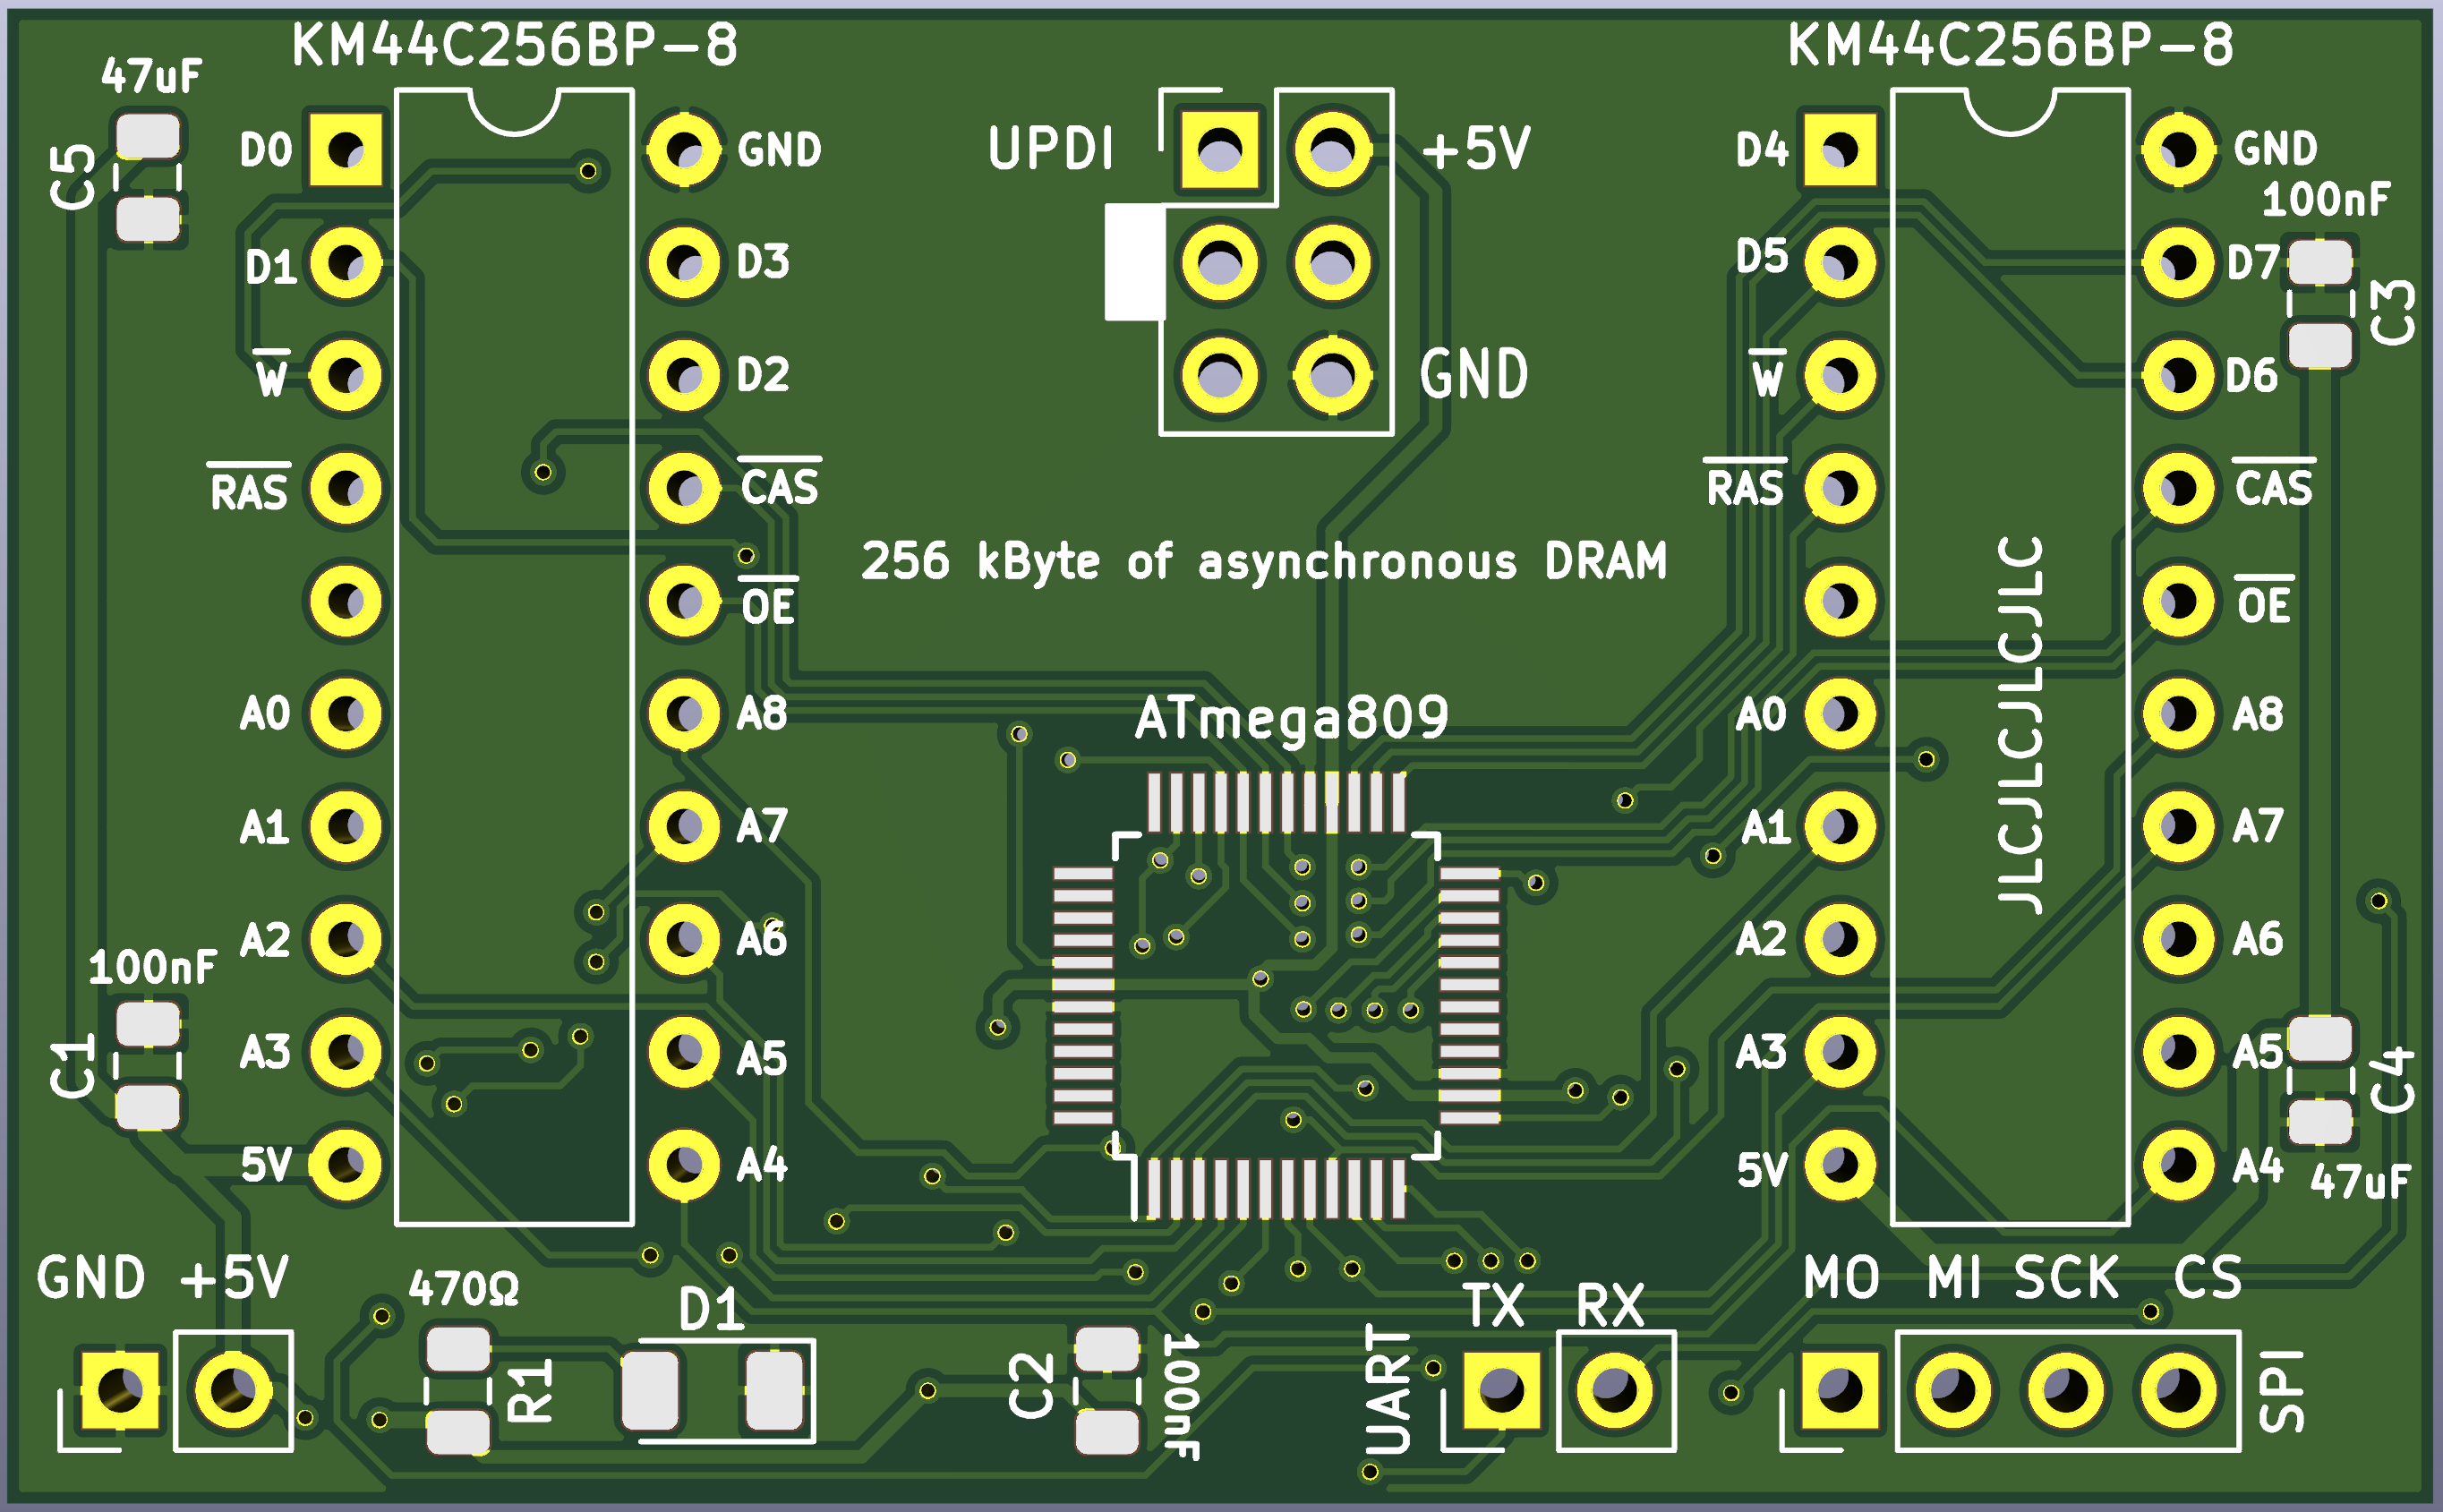
\includegraphics[scale=0.15]{images/KiCAD_3D_PCB_View.png}
	\end{center}
	
\end{frame}

\begin{frame}

	\frametitle{Das PCB}
	\framesubtitle{Fertige Platine}
	\begin{center}
		\includegraphics[scale=0.18]{images/PCB_assembled.png}
	\end{center}
	
\end{frame}

\begin{frame}

	\frametitle{KM44C256BP-8}
	\framesubtitle{}
	\begin{itemize}
		\item 9 Adresseingänge
		\begin{itemize}
			\item Werden sowohl für Spalten- als auch Zeilenadressen verwendet
			\item $2^{18} = 262144$ RAM-Zellen
		\end{itemize}
		\item 4 Dateneingänge
		\begin{itemize}
			\item Mit 2 Stück erhält man volle 256kByte
		\end{itemize}
		\item 8ms Refresh Period
		\item Asynchroner DRAM $\Rightarrow$ keinen Clock Eingang
		\item Neuere SDR-DRAM oder DDR-DRAM erfordern zu hohe Geschwindigkeiten
	\end{itemize}
	
\end{frame}

\begin{frame}

	\frametitle{KM44C256BP-8}
	\framesubtitle{READ}
	\begin{center}
		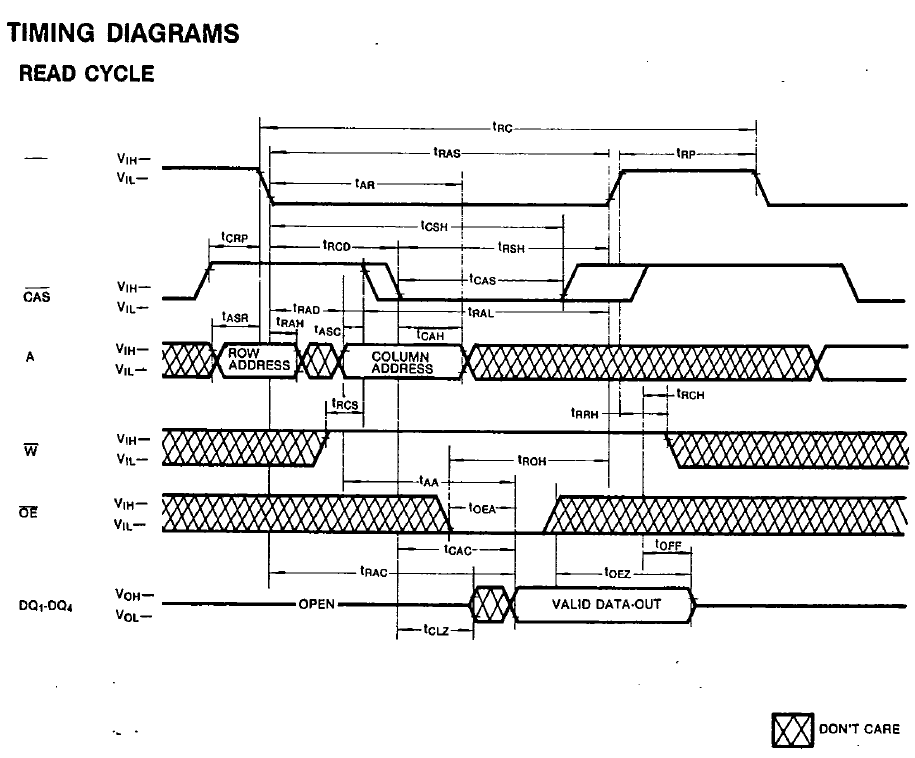
\includegraphics[scale=0.35]{images/DRAM_Read_Cycle.png}
	\end{center}
	
\end{frame}

\begin{frame}

	\frametitle{KM44C256BP-8}
	\framesubtitle{WRITE}
	\begin{center}
		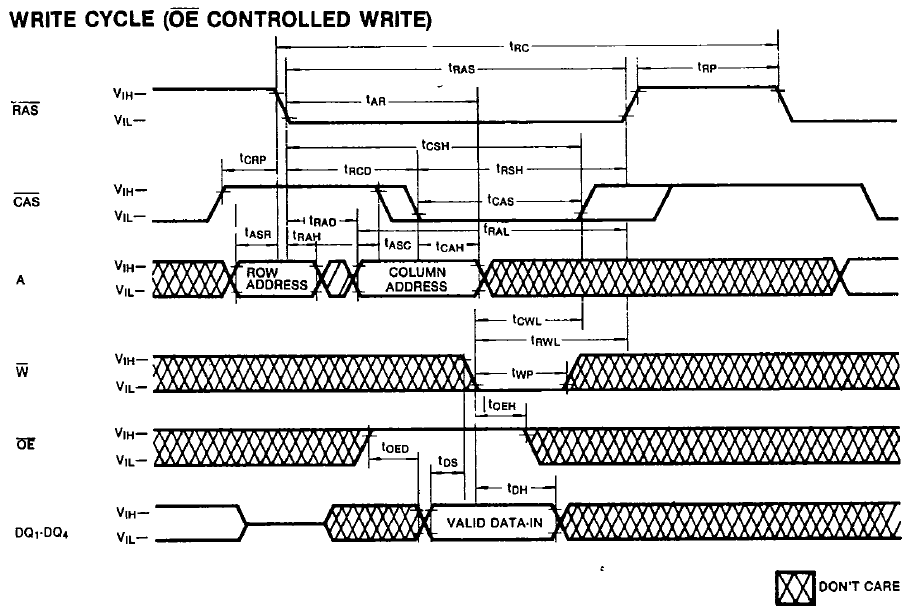
\includegraphics[scale=0.35]{images/DRAM_Write_Cycle.png}
	\end{center}
	
\end{frame}

\begin{frame}

	\frametitle{KM44C256BP-8}
	\framesubtitle{Refresh}
	\begin{center}
		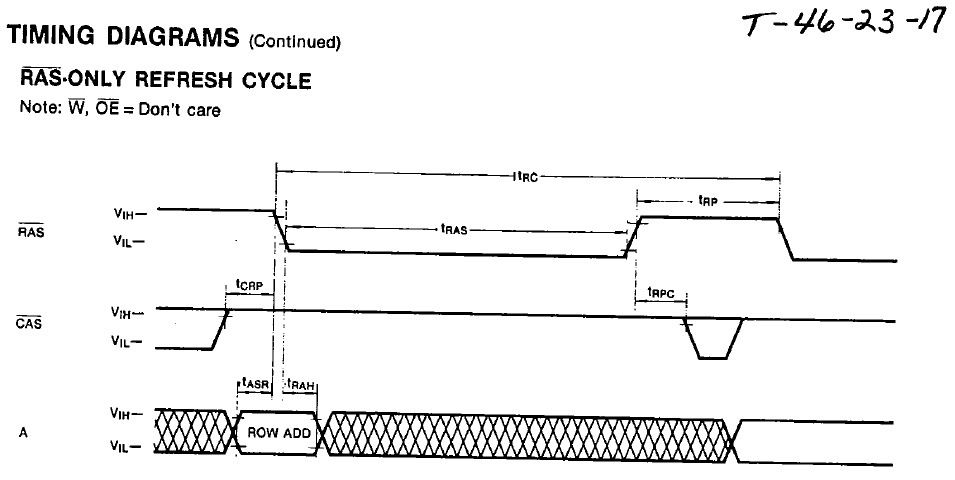
\includegraphics[scale=0.35]{images/DRAM_Refresh_Cycle.png}
	\end{center}
	
\end{frame}

\begin{frame}

	\frametitle{ATmega809}
	\framesubtitle{}
	\begin{itemize}
		\item Reagiert auf eintreffende SPI-Bytes
		\item Erkennt READ bzw. WRITE Befehle, steuert Adress- und Datenleitungen zum RAM entsprechend
		\item Führt zyklische $\bar{RAS}$-Refreshes aus
	\end{itemize}
	
\end{frame}

\begin{frame}[containsverbatim]

	\frametitle{ATmega809}
	\framesubtitle{}
	\begin{lstlisting}[style=CStyle]
int main(void) {
	initDRAMHandler(&dramHandler);

	initCPU();
	initSPI();
	initTimer0();
	
	while (1) {
		if(dramHandler.hasPendingRefresh) {
			dramHandler.refreshRASonly(&dramHandler);
			dramHandler.hasPendingRefresh = false;
		}
		if(dramHandler.hasPendingBufferUpdate) {
			dramHandler.processAndRespondBuffer(&dramHandler);
			dramHandler.hasPendingBufferUpdate = false;
		}
	}
}
	\end{lstlisting}
	
\end{frame}

\begin{frame}[containsverbatim]

	\frametitle{ATmega809}
	\framesubtitle{}
	\begin{lstlisting}[style=CStyle]
ISR(TCA0_CMP0_vect) {
	dramHandler.hasPendingRefresh = true;

	/* Clear interrupt flag */
	TCA0.SINGLE.INTFLAGS |= (1 << TCA_SINGLE_CMP0EN_bp);
}

ISR(SPI0_INT_vect) {
	if(SPI0.INTFLAGS & SPI_RXCIE_bm) {
		const uint8_t data = SPI0.DATA;
		dramHandler.buffer.push(&dramHandler.buffer, data);
		dramHandler.hasPendingBufferUpdate = true;
	}
}
	\end{lstlisting}
	
\end{frame}

\begin{frame}

	\frametitle{ESP8266}
	\framesubtitle{}
	\begin{itemize}
		\item Der ESP8266 agiert als SPI-Master
		\item Reagiert auf HTTP-Requests
		\item Sendet ggf. \textit{READ}/\textit{WRITE}-Befehle an ATmega809
		\item Zeigt Ergebnisse von READ-Befehlen an
	\end{itemize}
	
\end{frame}

\begin{frame}

	\frametitle{ESP8266}
	\framesubtitle{WRITE-Befehl}
	\begin{itemize}
		\item Besteht aus \[0x12, ADDR\_MSB, ADDR\_MLSB, ADDR\_LSB, DATA\]
	\end{itemize}
	\begin{center}
		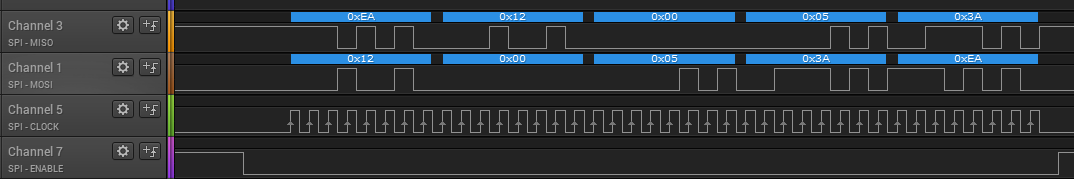
\includegraphics[scale=0.4]{images/SPI_Write_CMD_capture.png}
	\end{center}
	
\end{frame}

\begin{frame}

	\frametitle{ESP8266}
	\framesubtitle{READ-Befehl}
	\begin{itemize}
		\item Besteht aus \[0x13, ADDR\_MSB, ADDR\_MLSB, ADDR\_LSB\]\\ \[RET\_VAL\]
	\end{itemize}
	\begin{center}
		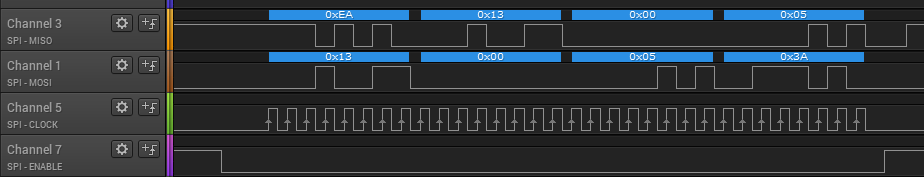
\includegraphics[scale=0.4]{images/SPI_Read_CMD_capture_01.png}
		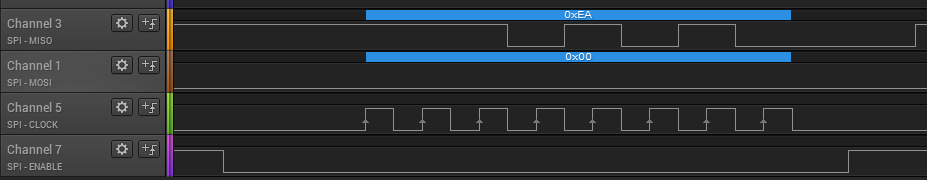
\includegraphics[scale=0.4]{images/SPI_Read_CMD_capture_02.png}
	\end{center}
	
\end{frame}

\begin{frame}

	\frametitle{ESP8266}
	\framesubtitle{Web-API}
	\begin{itemize}
		\item 192.168.4.1/get?addr=xxxxxx setzt READ-Befehl per SPI ab
		\begin{itemize}
			\item Zeigt ausgelesenen Wert auf der Webseite an
		\end{itemize}
		\item 192.168.4.1/set?addr=xxxxxx\&value=yyy setzt WRITE-Befehl per SPI ab
	\end{itemize}
	
\end{frame}

\usebeamertemplate{endpage}


\end{document}